% vim: set tw=0:
\documentclass{beamer}
\usepackage{graphicx}

% Reasonable themes:
% Antibes Bergen Berkeley Berlin Frankfurt Goettingen Ilmenau Luebeck Malmoe
% Montpellier PaloAlto Rochester Singapore Szeged Warsaw bars boxes
% compatibility default lined plain shadow sidebar split tree
% And these ones include the author's name on every slide:
% Berkeley

% Declare themes.
\mode<presentation>
\usetheme{UWHEP}

% Personal macros.
\newcommand{\email}[1]{{\texttt #1}}
\newcommand{\newframe}[1]{\section{#1}
    \frametitle{\sc{#1}}}
\newcommand{\subframe}[1]{\subsection{#1}
    \frametitle{\sc{#1}}}
\newcommand{\supers}[1]{\ensuremath{^\textrm{#1}}}
\newcommand{\subs}[1]{\ensuremath{_\textrm{#1}}}
\newcommand{\ca}{\ensuremath{\sim}}

% Author information.
\title{T2 Status}
\author[Maier, Mohapatra]{
    Will Maier \and Ajit Mohapatra\\ 
    {\tt wcmaier@hep.wisc.edu}\\
    {\tt ajit@hep.wisc.edu}}
\institute[Wisconsin]{University of Wisconsin - High Energy Physics}
\date{\today}
\logo{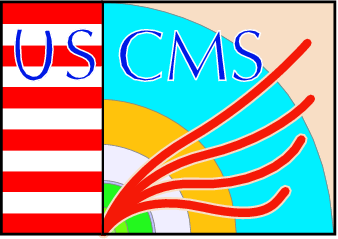
\includegraphics[height=0.6cm]{../../../Graphics/USCMS_logo.png}\hspace{.1cm}
\includegraphics[height=0.75cm]{../../../Graphics/UW_logo.png}}

\begin{document}

% http://indico.cern.ch/conferenceDisplay.py?confId=31476
% 283104
% 626 395 2112

\begin{frame}
    \titlepage
\end{frame}

%\section{Overview}
%\begin{frame}
%    \tableofcontents
%\end{frame}

\section{Facilities}
\subsection{Software and Storage}
\begin{frame}
\frametitle{}
\begin{itemize}
    \item Very brief unplanned PNFS outage 22 March, \ca{} 12:00 CST
    \begin{itemize}
        \item No indication of core problem
        \item Slight delay; init scripts weren't starting {\tt pnfs}
    \end{itemize}
    \item DNS outage 29 March, \ca{} 10:00 - 11:00 CST
    \begin{itemize}
        \item Lost several decommissioned servers simultaneously
        \item Also lost primary DNS; brought up backup server
    \end{itemize}
    \item Completed spring hardware purchase
    \begin{itemize}
        \item 32 1U nodes, 128 TB, 256 CPUs @ 3.0 GHz (Xeon E5450)
        \item Hope to test and deploy by early May
    \end{itemize}
    \item New dCache hardware deployment
    \begin{itemize}
        \item Planned outage for 07:00 - 17:00 CST tomorrow (2 April)
        \item Replace all core dCache hardware
        \item Had planned for later in April, but admin server started showing disk problems
        \item Also rearranging other nodes on the main CMS rack (better use UPS)
    \end{itemize}
    \item Debugged another CMSSW installation problem; switching target node
\end{itemize}
\end{frame}

\subsection{Production and Monitoring}
\begin{frame}
\frametitle{}
\begin{itemize}
    \item SAM: OK
    \item JobRobot: OK
    \item LoadTest:
    \begin{itemize}
        \item Debugging RAL/Wisconsin link (DDT2)
        \item Production data subscribed for local users/HLT validation
    \end{itemize}
    \item MC Production:
    \begin{itemize}
        \item CSA07 production nearly done
        \item Testing new PA features to get ready for CSA08
    \end{itemize}
\end{itemize}
\end{frame}

\end{document}
